\section{Evaluation}
\label{sec:evaluation}

We evaluate \tool optimizations by comparing the performance of three programs: \emph{i)} A word count with prior text parsing, \emph{ii)} TPCH \cite{tpch} query 12 and a  \emph{iii)} k-means application. To evaluate the extensibility of the framework we introduce a new DSL component that represents vectors in the k-means benchmark.

All experiments were performed on the Amazon EC2 Cloud, using 20 "m1.large" nodes as slaves and one as a master. They each have 7.5 GB of memory, 2 virtual cores with 2 EC2 compute units each, 850 GB of instance storage distributed over 2 physical hard drives and have 1 Gb/s network interface. Prior to the experiments we have measured up to 50 MB/s between two nodes. For the Hadoop experiments we used the cdh3u4 Cloudera Hadoop distribution. On top of it we used Crunch version 0.2.4 and Scoobi 0.4.0. We did not tweak Hadoop configuration beyond the default settings set by the Whirr 0.7.1 \todo{cite} tool. For benchmarking Spark we used the Mesos \cite{hindman_mesos:_2011} EC2 script to start a cluster, and the most recent version of Spark for our tests. For Spark we changed the default parallelism level to the number of cores in the cluster and increased the maximum memory to 6GB. 

% Regular expressions
While doing preliminary benchmarking we found some easy tweaks focused on regular expressions that we needed to include in \tool in order to have a fair comparison against Pig, which contains them. We implemented a fast splitter, which uses an efficient character comparison whenever the regular expression allows this. Additionally we select based on the regular expression between Java's implementation and the automaton library \cite{mollerdk}.
%For a fairer comparison with Pig we adapted some of their regular expression optimizations for our program. Pig makes use of a faster library \cite{mollerdk} and implements an optimized splitting function when the regular expression becomes a simple comparison of one character. We implemented a frontend for regular expressions which automatically selects the best variant for each expression and operation. 

% Data Serialization
For serialization of data we used LMS code generation to achieve minimal overhead for both Crunch and Scoobi frameworks because they outperformed the Kryo \todo{cite kryo} library by a small margin. For Spark we used the standard serialization mode which uses Kryo. All benchmarks were run three times and in the figures we present the average value. We also computed the standard deviations but we omitted them since they are smaller than 3\% in all the experiments.

\todo{code for all benchmarks and generated program versions can be found }

\begin{figure}[!hbt]
    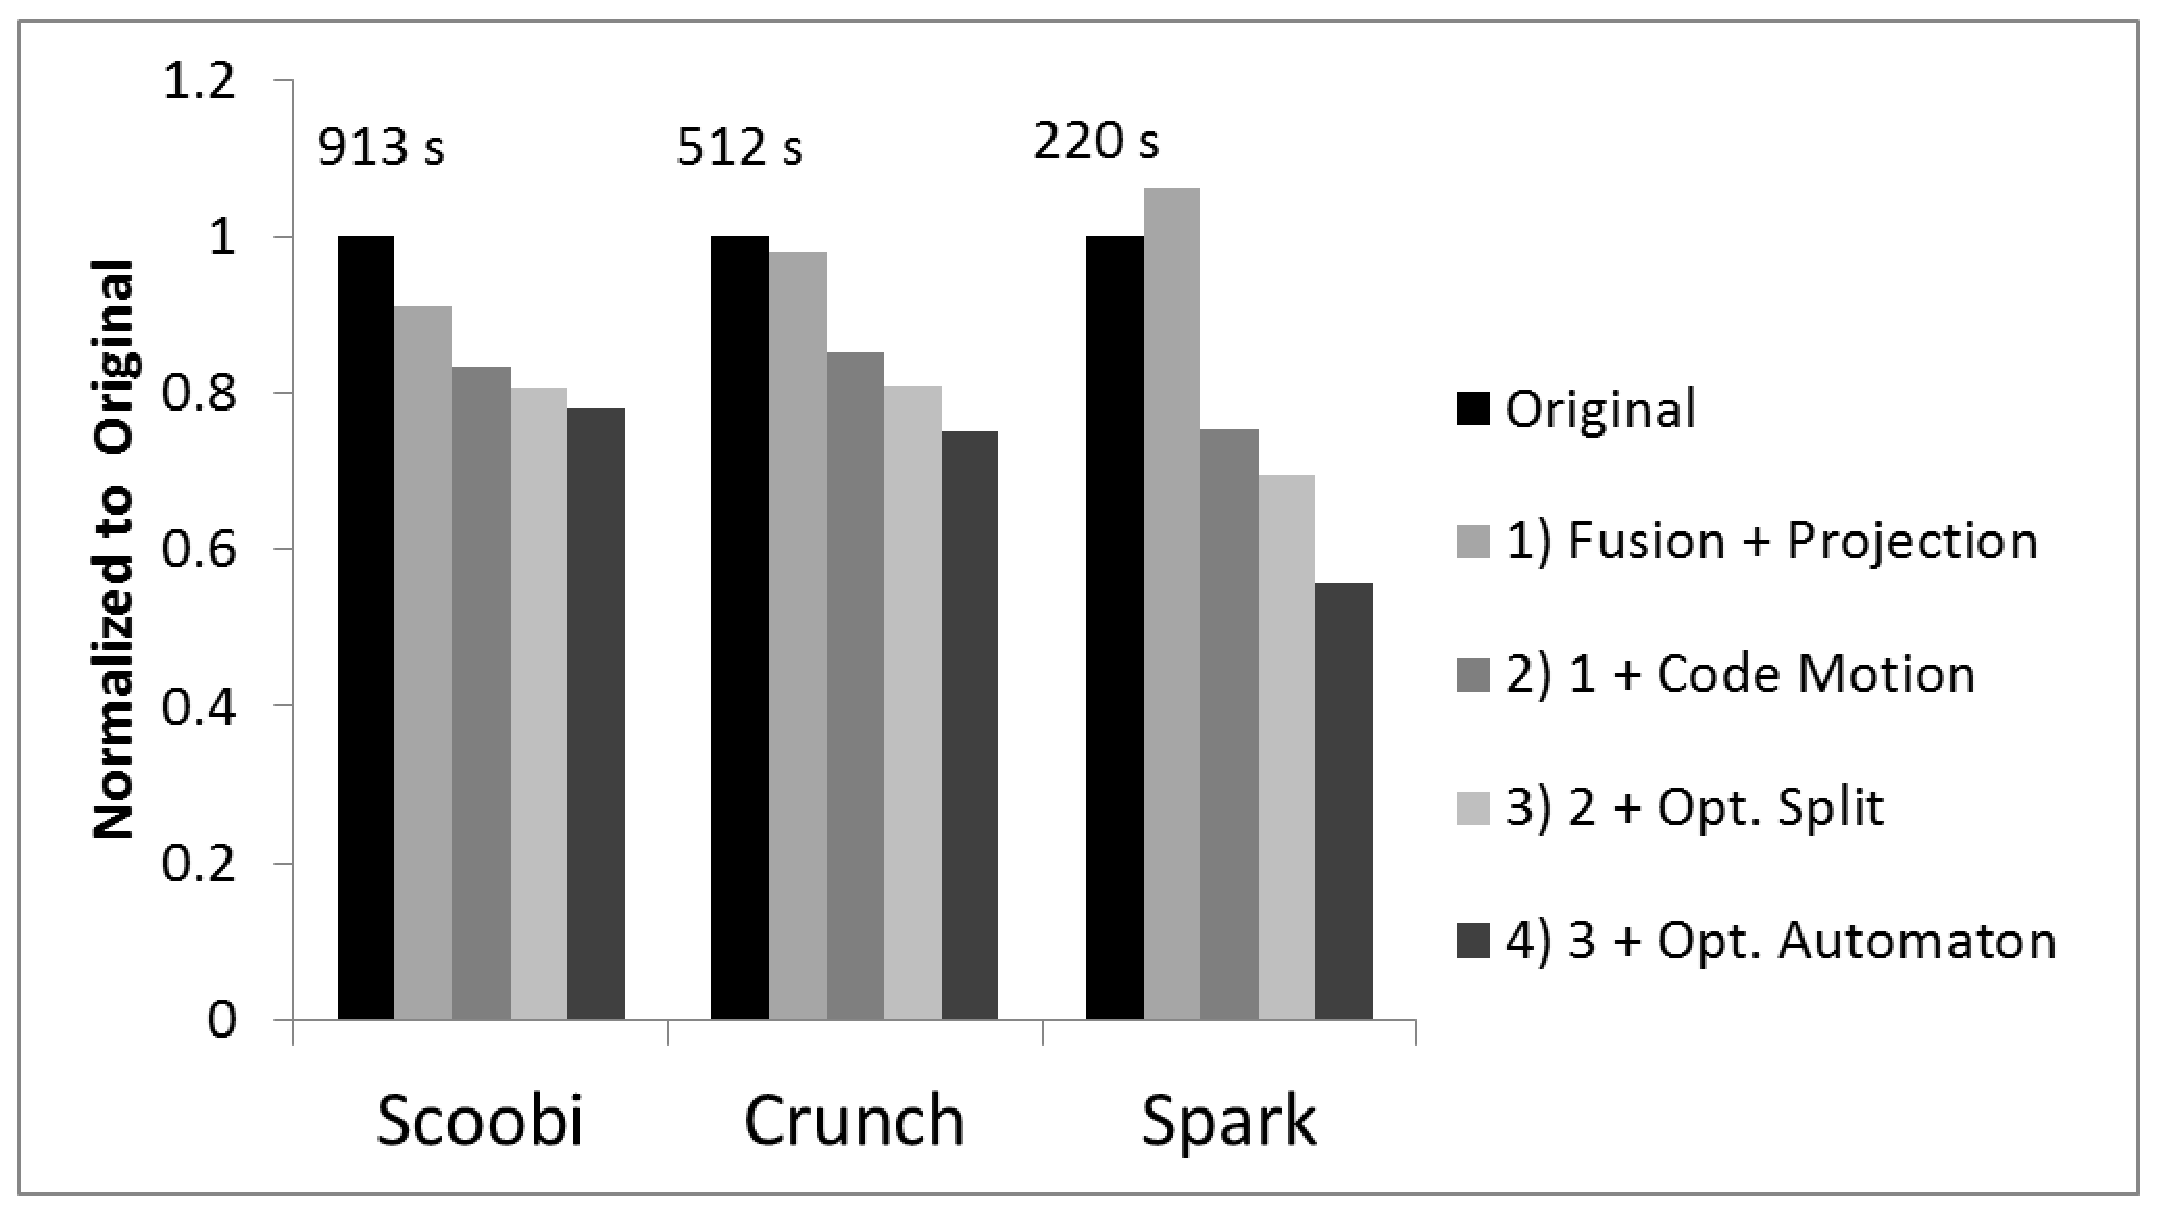
\includegraphics[width=8.6cm]{figures/word-count}
   \caption{Word Count benchmark.}
   \label{fig:word-count}%\vspace{10pt}
\end{figure}

\begin{figure}[!hbt]
    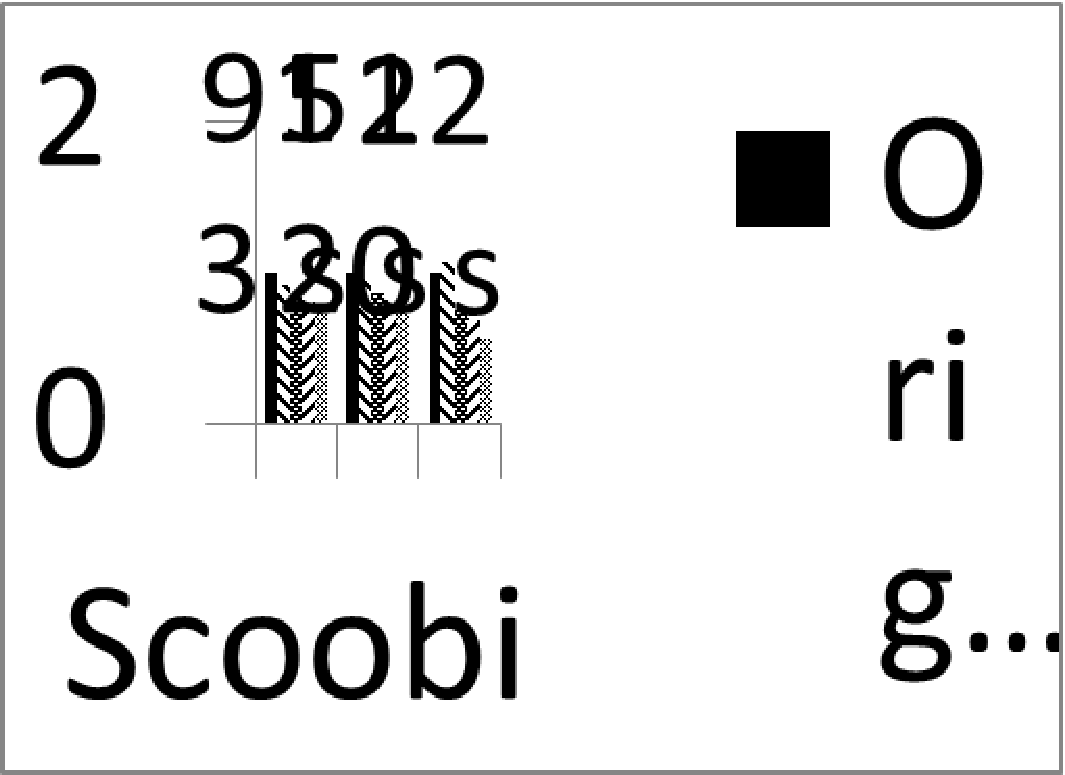
\includegraphics[width=8.6cm]{figures/k-means}
   \caption{K-means benchmark.}
   \label{fig:k-means}%\vspace{10pt}
\end{figure}

\begin{figure}[!hbt]
    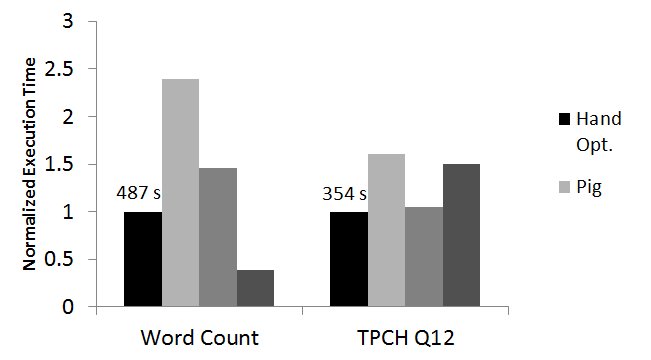
\includegraphics[width=8.6cm]{figures/pig}
   \caption{Comparison between Pig, Scoobi, Spark and Crunch.}
   \label{fig:pig}%\vspace{10pt}
\end{figure}

\begin{figure}[!hbt]
    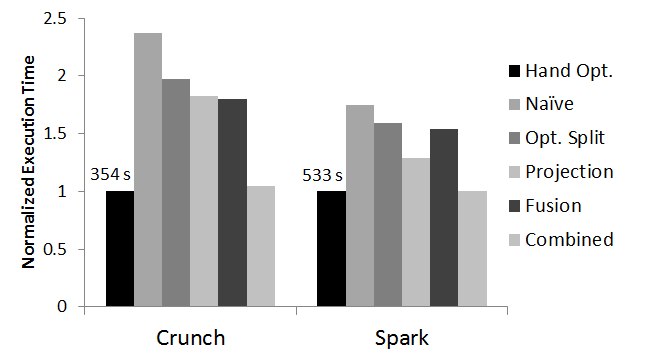
\includegraphics[width=8.6cm]{figures/tpch}

   \caption{TPCH query 12 benchmark.}
  \label{fig:tpch}%\vspace{10pt}    
\end{figure}

% WordCount
\subsection{Parsing and Word Count}
\label{subsec:parsing-word-count}

In this benchmark we evaluate the performance of \tool compiler optimizations without focusing on projection insertion. We choose a word count application that, prior to the inexpensive network shuffle, parses the input with 5 regular expressions making this job CPU bound. For this evaluation we start with an the original version of the program and add optimizations one by one. We first add the operation fusion and projection insertion optimizations. We then include code motion that removes regular expression compilation out of hot loops. Next we add the fast splitter and for the fully optimized version we use the optimized automaton regular expression library.    

Our input is a 62 GB set of plain text version of Freebase Wikipedia articles. Our regular expressions are used clean up articles from strings that are not text words. This benchmark does not benefit from projection insertion but we include it for the comparison with the Pig framework in subsection \ref{subsec:pig}.

In figure \ref{fig:word-count} we show the job times for these versions normalized to the original program version. Performance improvements of all optimizations combined are from 29\% for Scoobi, 33\% for Crunch and 79\% for Spark. The base performance of the frameworks differ by a large margin for this benchmark. Scoobi profits the most in this case from the fusion which indicates that the framework imposes additional overhead for declarative operations. In Spark, we notice larger benefits from our optimizations. We argue that it has significantly smaller IO overhead so that the optimizations have a bigger impact. Also, we notice that fusion optimization with projection insertion is slower than the original program for Spark. This result does not match our experiments in a smaller cluster setup, we believe that it could be caused by a straggler node in the cloud environment.

% TPCH q12
\subsection{TPCH Query 12}
\label{subsec:tpch-query-12}

This benchmark evaluates all optimizations combined but emphasizes the projection insertion. We chose the TPCH query 12 which includes an expensive \code{join} operation after which only two columns of the original data are used, thus giving projection insertion opportunity to eliminate unused columns. We compare the original program to each optimizations separately and all of them combined. As the data set we use a 100 GB plain text input generated by the DbGen tool \cite{tpch}.

In figure \ref{fig:tpch} we show job times for different optimizations normalized to the original program version on different frameworks. We notice that projection insertion gives 20\% percent better performance on Crunch and 11\% on Scoobi. On Spark, the projection insertion improves the performance by 40\%, significantly more than for the Hadoop based frameworks. We believe the difference is caused by Hadoop spills of the data to disk earlier, while Spark tries to keep it in the memory before it spills it. Spark is therefore very sensitive to memory overhead of the large \code{join}.

%We believe that either network shuffle or the \code{join} operation are less optimal in Spark. 
In this benchmark the optimizations interact with each other. The absolute performance gain for combined optimizations is 3\% greater for Crunch, equal for Scoobi and 9\% smaller for Spark than the sum of the absolute individual gains.

\subsection{Comparison with Pig}
\label{subsec:pig}

% Pig Comparison
In figure \ref{fig:pig} we compare the most optimal versions of benchmarks to equivalent Pig programs. The figure is normalized to the Pig execution time and overall job time is stated above the bar. We notice that for TPCH query 12 the combination of fusion, code motion and field reduction outperform Pig when the Crunch framework is used. 

% Spark
For the sake of showing comparison between the Hadoop based frameworks and the Spark framework we include the Spark results in the graph. We see that in all cases except for unoptimized TPCH query 12 it significantly outperforms the Hadoop based frameworks.

In the word count benchmark Crunch outperforms Pig even without any optimizations applied. We believe that Pig uses inefficiency string processing primitives. With all optimizations Crunch is 73\% faster than Pig. We explain this by the more optimal regular expressions processing support included in the \tool. In regular expressions used in the benchmark Pig falls back to default Java regular expressions while \tool uses optimized automaton library. Scoobi framework performs slower than Pig in both benchmarks even with all optimizations applied.


\subsection{Extensibility and Modularity}
\label{subsec:kmeans}

To evaluate modularity and extensibility of \tool we decided to extend with a \code{Vector} abstraction that has abstract methods for arithmetic vector operations that get compiled into loops over arrays. We also chose this benchmark to emphasize the extensibility of \tool.
%say what the section does 
  % 1) test language extensibility, vector run on k-means 
  % 2) evaluate effort to support different backends

% K-means   
% language extensibility with KMeans
We took a version of Spark k-means program \todo{cite NSDI} application and ported it to our own language. This application can neither benefits from projection insertion reduction nor from operation fusion. We extended our DSL for this program with a highly optimized vector type that has all its operations iterating over the dimensions compiled into while loops. We only evaluate this benchmark on Spark, since it uses operations only defined in Spark and since it is known to outperform Hadoop by a large margin. As input we use synthetic data with 10 to 1000 dimensions, 100 centers and we keep the dimensions * points factor constant so that each input file is around 20Gb.

% Different backends
Our results are similar to those described by Murray et al. in \cite{murray_steno:_2011}. In lower dimensions our optimization shows large speedup while for 1000 dimensions our version performs slightly worse. We believe that the iterator overhead is quite high in case of 10 dimensions, such that our loops which removes it performs much better. At higher dimensions it's possible that the JVM can do a better job optimizing if the code is smaller, such that our pre optimized and larger code becomes slightly slower. In any case our implementation seems favorable as it performs more consistently for different dimensions.

%We were also getting unsatisfying numbers from our Scoobi backend, so we added Crunch in about one week. This really shows that it is easy to add a new backend, and the modularity allows us to reuse pieces of other backends. Crunch's implementation of join performed very badly in local benchmarks, so we replaced it with our own one for these benchmarks.
%The independence of code generation from the optimizations is confirmed by the fact that our implementations for the backends are very small in terms of code size, ranging from 270 to 425 lines of code.